\chapter{Auger Decay of Noble Gas Atoms}
\section{Neon}

\begin{table}[h]
  \centering
  \caption{Auger decay widths and percentages of the partial decay widths
           for a initial vacancy in the Ne1s. The decay widths are given in
           \unit[]{meV}.}
  \small
  \begin{tabular}{llrrrrrrrrrrrr}
   \toprule
    & & \multicolumn{4}{c}{Present} & \multicolumn{2}{c}{Koloren\v{c}} & \multicolumn{2}{c}{Kelly} & \multicolumn{2}{c}{Yarzhemsky} & \multicolumn{2}{c}{exp.}\\
   \multicolumn{2}{c}{Final states} & \multicolumn{2}{c}{rel.} & \multicolumn{2}{c}{nrel.} & \multicolumn{2}{c}{Ref.\cite{Kolorenc11}} & \multicolumn{2}{c}{Ref.\cite{Kelly75}} & \multicolumn{2}{c}{Ref.\cite{Yarzhemsky02}} & \multicolumn{2}{c}{Refs. \cite{Albiez90}, \cite{Avaldi95}}\\
   \midrule
   \multirow{3}{*}{2p$^{-2}$} & $^3P$ &  & \multirow{3}{*}{53.9} & 0.0 & \multirow{3}{*}{81.6} &  0.0 & \multirow{3}{*}{60.0} &  0.0 & \multirow{3}{*}{70.8} &  0.0 & \multirow{3}{*}{68.4} &  --  & \multirow{3}{*}{70.4}\\
                              & $^1D$ &     & & \multirow{2}{*}{81.6} & & 50.5 & & 61.2 & & 58.2 & & 60.9&\\
                              & $^1S$ &     & &  & &  9.5 & &  9.6 & & 10.2 & &  9.5&\\
   \midrule
 \multirow{2}{*}{2s$^{-1}$2p$^{-1}$} & $^3P$ &    & \multirow{2}{*}{38.0} & 1.1 & \multirow{2}{*}{7.8} & 10.6 & \multirow{2}{*}{30.1} &  6.1 & \multirow{2}{*}{23.1} &  9.3 & \multirow{2}{*}{26.1} &  6.3 & \multirow{2}{*}{23.5}\\
                              & $^1S$ &      & &  6.8 & & 19.5 & & 17.0 & & 16.8 & & 17.2&\\
   \midrule
      2s$^{-2}$               & $^1S$ &      & 8.1 & 10.4 & 10.4 &  9.9 & 9.9 &  6.1 & 6.1 &  5.5 & 5.5 &  6.1& 6.1\\
   \midrule
   $\Gamma$  & & \multicolumn{2}{c}{344}  & \multicolumn{2}{c}{268} & \multicolumn{2}{c}{251} & \multicolumn{2}{c}{219} & \multicolumn{2}{c}{242} & \multicolumn{2}{c}{220 $\pm$ 30}\\
   \bottomrule
  \end{tabular}
  \label{table:Ne_gammas}
\end{table}

\section{Xenon}
From single and double ionization spectra and Auger spectroscopy
it is known, that vacancies from the Xe4d and lower are energetically allowed to
decay via Auger processes. \cite{Siegbahn69}
I will in the following focus on two energetic initial state regions, namely
the 4p and the 4d region.

The different open channels have to be determined by comparison of the single
and double ionization spectra shown in figure \ref{figure:Xe_sdip}.
These spectra have been calculated using the
DC-ADC(2x) implemented in Dirac\cite{Pernpointner04_1,Pernpointner10_1,DIRAC13}.
All calculations in this chapter were performed 
Dyall cv4z basis set\cite{dyall5p06} with additional five s, p and d
and three diffuse basis functions                       
of the \ac{KBJ} type \cite{Kaufmann89}.

\begin{figure}[h]
  \centering
  \begin{tikzpicture}[scale=1.0]

\begin{axis}[%scale=1.5,
             domain=30:170,
             %y domain=1E-8:10,
             restrict expr to domain={x}{30:170},
             xlabel={E in \unit{eV}},
             xtick={30,50,...,170},
             %xticklabels={2,4,6,8,10,12,15,20,25},
             ytick={-1.0,-0.8,...,1.0},
             yticklabels={1.0,0.8,0.6,0.4,0.2,0.0,0.2,0.4,0.6,0.8,1.0},
             ylabel={pole strength},
             scale only axis,
             width=\textwidth-2cm,
             height=7cm
             %title={Parameter Fitting of NeNe and NeAr Decay Widths}
             ]

\draw[gray]
  (axis cs:\pgfkeysvalueof{/pgfplots/xmin},0) --
  (axis cs:\pgfkeysvalueof{/pgfplots/xmax},0);
\addplot+[ycomb,
         %no markers,
         mark=.,
         thick,
         diplom1,
         forget plot
        ]
        table[
        x expr = \thisrowno{0},
        y expr = \thisrowno{1}
        ]
        {data/Xe_rel_sips.dat};
        \addlegendimage{line legend, diplom1, thick};
        \addlegendentry{SIPs(Xe)};
\addplot+[ycomb,
         %no markers,
         mark=.,
         thick,
         diplom2,
         forget plot
        ]
        table[
        x expr = \thisrowno{0},
        y expr = -\thisrowno{1}
        ]
        {data/Xe_rel_dips.dat};
        \addlegendimage{line legend, diplom2, thick};
        \addlegendentry{DIPs(Xe)};

\node[pin={[pin distance=0.2cm]170:{\tiny 4d$_{5/2}^{-1}$}}]
     at (axis cs:67.03,0.6) {};
\node[pin={[pin distance=0.2cm]10:{\tiny 4d$_{3/2}^{-1}$}}]
     at (axis cs:69.06,0.6) {};
\node[pin={[pin distance=0.2cm]170:{\tiny 4p$_{3/2}^{-1}$}}]
     at (axis cs:146.6,0.2) {};
\draw[] (axis cs:165,0.15) arc [radius=0.75cm,start angle=10,end angle=100];
\node[pin={[pin distance=0.2cm]20:{\tiny 4p$_{1/2}^{-1}$}}]
     at (axis cs:159.6,0.23) {};
 		
%DIPs
\draw[] (axis cs:39,-0.9) arc [radius=0.3cm,start angle=358,end angle=180];
\node[pin={[pin distance=0.10cm]95:{\tiny 5p$^{-2}$}}]
     at (axis cs:32,-0.75) {};

\draw[] (axis cs:50,-0.75) arc [radius=0.3cm,start angle=358,end angle=180];
\node[pin={[pin distance=0.05cm]280:{\tiny 5s$^{-1}$5p$^{-1}$}}]
     at (axis cs:47,-0.80) {};

\node[pin={[pin distance=0.1cm]350:{\tiny 5s$^{-2}$}}]
     at (axis cs:59,-0.35) {};

\draw[] (axis cs:96,-0.80) arc [radius=0.3cm,start angle=358,end angle=180];
\node[pin={[pin distance=0.05cm]270:{\tiny 4d$^{-1}$5p$^{-1}$}}]
     at (axis cs:91,-0.85) {};

\draw[] (axis cs:110,-0.70) arc [radius=0.3cm,start angle=358,end angle=180];
\node[pin={[pin distance=0.05cm]300:{\tiny 4d$^{-1}$5s$^{-1}$}}]
     at (axis cs:106,-0.75) {};

\draw[] (axis cs:165,-0.75) arc [radius=0.65cm,start angle=340,end angle=180];
\node[pin={[pin distance=0.05cm]260:{\tiny 4d$^{-2}$}}]
     at (axis cs:154,-0.80) {};

\end{axis}
\end{tikzpicture}

  \begin{tikzpicture}[scale=1.0]

\begin{axis}[%scale=1.5,
             domain=30:170,
             %y domain=1E-8:10,
             restrict expr to domain={x}{30:170},
             xlabel={E in \unit{eV}},
             xtick={30,50,...,170},
             %xticklabels={2,4,6,8,10,12,15,20,25},
             ytick={-1.0,-0.8,...,1.0},
             yticklabels={1.0,0.8,0.6,0.4,0.2,0.0,0.2,0.4,0.6,0.8,1.0},
             ylabel={pole strength},
             scale only axis,
             width=\textwidth-2cm,
             height=7cm
             %title={Parameter Fitting of NeNe and NeAr Decay Widths}
             ]

\draw[gray]
  (axis cs:\pgfkeysvalueof{/pgfplots/xmin},0) --
  (axis cs:\pgfkeysvalueof{/pgfplots/xmax},0);
\addplot+[ycomb,
         %no markers,
         mark=.,
         thick,
         diplom1,
         empty legend
        ]
        table[
        x expr = \thisrowno{0},
        y expr = \thisrowno{1}
        ]
        {data/Xe_nrel_sips.dat};
        \addlegendentry{SIPs(Xe)};
\addplot+[ycomb,
         %no markers,
         mark=.,
         thick,
         diplom2,
         empty legend
        ]
        table[
        x expr = \thisrowno{0},
        y expr = -\thisrowno{1}
        ]
        {data/Xe_nrel_dips.dat};
        \addlegendentry{DIPs(Xe)};

\node[pin={[pin distance=0.2cm]10:{\tiny 4d$^{-1}$}}]
     at (axis cs:69.06,0.6) {};
\draw[] (axis cs:155,0.41) arc [radius=0.5cm,start angle=10,end angle=100];
\node[pin={[pin distance=0.2cm]20:{\tiny 4p$^{-1}$}}]
     at (axis cs:152.0,0.43) {};
 		
%DIPs
\draw[] (axis cs:39,-0.9) arc [radius=0.2cm,start angle=358,end angle=180];
\node[pin={[pin distance=0.1cm]95:{\tiny 5p$^{-2}$}}]
     at (axis cs:32,-0.75) {};

\draw[] (axis cs:50,-0.70) arc [radius=0.2cm,start angle=358,end angle=180];
\node[pin={[pin distance=0.05cm]280:{\tiny 5s$^{-1}$5p$^{-1}$}}]
     at (axis cs:47,-0.75) {};

\node[pin={[pin distance=0.1cm]350:{\tiny 5s$^{-2}$}}]
     at (axis cs:55,-0.40) {};

\draw[] (axis cs:100,-0.80) arc [radius=0.22cm,start angle=358,end angle=180];
\node[pin={[pin distance=0.05cm]270:{\tiny 4d$^{-1}$5p$^{-1}$}}]
     at (axis cs:94,-0.85) {};

\draw[] (axis cs:111,-0.70) arc [radius=0.22cm,start angle=358,end angle=180];
\node[pin={[pin distance=0.05cm]300:{\tiny 4d$^{-1}$5s$^{-1}$}}]
     at (axis cs:107,-0.75) {};

\draw[] (axis cs:170,-0.75) arc [radius=0.45cm,start angle=340,end angle=180];
\node[pin={[pin distance=0.05cm]260:{\tiny 4d$^{-2}$}}]
     at (axis cs:156,-0.80) {};

\end{axis}
\end{tikzpicture}

  \caption{Comparison of calculated single and double ionization spectra
           for the determination of open channels in of the later decay
           width calculation. Upper panel: relativistic description, lower
           panel: non-relativistic description.
           }
  \label{figure:Xe_sdip}
\end{figure}
\afterpage{\clearpage}


Therefore the channels shown in table \ref{table:Xe_open_channels} are
open for the different initial states. For the decay width calculations, these
results are the basement for the choice of the final state subspace.
\begin{table}[h]
  \centering
  \caption{Open channels of the Auger processes for different initial states
           on the xenon atom.}
  \begin{tabular}{lcccccc}
   \toprule
                   & 4d$^{-2}$ & 4d$^{-1}$5s$^{-1}$ & 4d$^{-1}$5p$^{-1}$ & 5s$^{-2}$ & 5s$^{-1}$5p$^{-1}$ & 5p$^{-2}$ \\
   \midrule
   4d$_{5/2}^{-1}$ &      --   &       --           &        --          &     x     &     x              &     x     \\
   4d$_{3/2}^{-1}$ &      --   &       --           &        --          &     x     &     x              &     x     \\
   4p$_{3/2}^{-1}$ &      --   &        x           &         x          &     x     &     x              &     x     \\
   4p$_{1/2}^{-1}$ &       x   &        x           &         x          &     x     &     x              &     x     \\
   \midrule
   4d$^{-1}_{nrel}$&      --   &       --           &        --          &     x     &     x              &     x     \\
   4p$^{-1}_{nrel}$&      --   &        x           &         x          &     x     &     x              &     x     \\
   \bottomrule
  \end{tabular}
  \label{table:Xe_open_channels}
\end{table}




\subsection{Auger Decay from the Xe4d Region}

The Auger process from the Xe4d subshell has been experimentally
measured to high accuracy and is used as a calibration standard. \cite{Carroll02}
The decay widths have been measured e.g. Ausmees \textit{et al.}
\cite{Ausmees99,Aksela94}
Theoretically it has been investigated  by Mäntykenttä \cite{Maentykenttae93}
and lately as a competing process for
sequential double ionization using a free electron laser \cite{Fritzsche11}
using \ac{MCDF}. 
We are going to compare the experimental and theoretical findings with our 
the results from our calculations presented in table \ref{table:xe_auger_4d_rates}.

From the single ionization spectrum of the full Hamiltonian, initial state
energies of \unit[67.03]{eV} and \unit[69.04]{eV} were obtained. They deviate
from the experimental values shown in \ref{table:xe_auger_4d_rates}
by about \unit[0.5]{eV} and are very close to the values calculated with
\ac{MCDF} \cite{Fritzsche11}. However, the spin-orbit splitting of
$\Delta_{SO,calc}=\unit[2.01]{eV}$ is very close to the experimental value
of $\Delta_{SO,exp}=\unit[1.99]{eV}$. Even though the initial state energies of the
initial state subspace deviates from the experimental numbers, the spin-orbit
splitting is well preserved to be $\Delta_{SO,part}=\unit[2.04]{eV}$.

The open final state channels as summarized in table
\ref{table:Xe_open_channels} are $5s^{-2}$, $5s^{-1}5p^{-1}$ and $5p^{-1}5p^{-1}$.


In order to obtain the decay widths at the resonant energies,
higher orders of Stieltjes (15 -- 38) were predominantely
used for the interpolation to yield the approximate decay width function.
It became necessary, because in the partitioned Hamiltonian the $5s^{-2}$ channel
opens very close to threshold and hence the resonance energy at which the decay width
function is evaluated is very steep. Therefore, for a reasonable description,
the higher orders were needed. In such cases also the error of the evaluated decay width 
is rather
large compared to the decay widths themselves being $\Delta(\Gamma)=\unit[0.1]{eV}$.

\begin{table}[h]
 \centering
 \footnotesize
 \caption{Auger decay widths of the Xe4d$_{3/2}$ and Xe4d$_{3/2}$
          and the non-relativistic
          4d compared to experimental values\cite{Ausmees99}.
          All widths are given in \unit{eV}.
          The partial widths are renormalized to the total width.}
 \begin{tabular}{lcccccc}
   \toprule
               & energy [\unit{eV}] & pole strength & $5s^{-2}$          & $5s^{-1}5p^{-1}$   & $5p^{-1}5p^{-1}$   & total \\
   \midrule                                                                                     
     4d$_{5/2,\pm 5/2}$ &  66.87    &   0.879       & 2.34$\cdot10^{-2}$ & 5.40$\cdot10^{-2}$ & 8.45$\cdot10^{-2}$ & 0.1619 $\pm$ 0.1\\
     4d$_{5/2,\pm 3/2}$ &  66.87    &   0.879       & 2.30$\cdot10^{-2}$ & 5.34$\cdot10^{-2}$ & 8.57$\cdot10^{-2}$ & 0.1621 $\pm$ 0.1\\
     4d$_{3/2,\pm 3/2}$ &  68.91    &   0.879       & 1.73$\cdot10^{-2}$ & 3.35$\cdot10^{-2}$ & 8.15$\cdot10^{-2}$ & 0.1323 $\pm$ 0.1\\
     4d$_{3/2,\pm 1/2}$ &  68.91    &   0.879       & 1.62$\cdot10^{-2}$ & 3.21$\cdot10^{-2}$ & 8.21$\cdot10^{-2}$ & 0.1304 $\pm$ 0.1\\
     4d$_{spinfree}$    &  67.67    &   0.879       & 2.29$\cdot10^{-2}$ & 5.17$\cdot10^{-2}$ & 9.31$\cdot10^{-2}$ & 0.1678 $\pm$ 0.1\\
     4d$_{nrel}$        &  70.68    &   0.878       & 1.15$\cdot10^{-2}$ & 1.78$\cdot10^{-2}$ & 5.72$\cdot10^{-2}$ & 0.0898 $\pm$ 0.1\\
     \midrule
     exp. 4d$_{5/2}$    &  67.55 \cite{King77}   &      &       &   &    & 0.110 -- 0.130 \cite{Ausmees99} \\
     exp. 4d$_{3/2}$    &  69.54 \cite{King77}   &      &       &   &    & 0.105 -- 0.116 \cite{Ausmees99} \\
     calc. 4d$_{5/2}$ \cite{Maentykenttae93} &67.55&    &       &   &    & 0.160  \\
     calc. 4d$_{3/2}$ \cite{Maentykenttae93} &69.54&    &       &   &    & 0.143  \\
   \bottomrule                                                                                 
 \end{tabular}                                                                                 
 \label{table:xe_auger_4d_rates}
\end{table}

The total decay width obtained with the FanoADC Stieltjes method agree with
both the experimental results and the \ac{MCDF} result within the error margins.
Even though the error margins are large, the deviation of the results
from the experimental findings are
less than \unit[52]{meV} and hence much smaller than the error margin. 
Compared to the \ac{MCDF} the deviations are much smaller, for the 4d$_{5/2}$
the results are very close with a difference of \unit[2]{meV} and for the
4d$_{3/2}$ with a difference of \unit[10]{meV}.


As shown in figure \ref{figure:Xe_sdip}, some of the final state groups
split into different terms which have been thoroughly analyzed by
Pernpointner \textit{et al.} \cite{Pernpointner12_2}. From this analysis
it can easily be seen that the terms are combinations of different $2h$
configurations. Therefore a definition of the final state by $2h$
configurations is unfortunately insufficient for a more detailed
study of partial decay widths.
However, the Auger process from the Xe4d region with an improved method
would be worth investigating, since decay width and branching ratios have been
measured experimentally. \cite{Aksela94}




\subsection{Auger Decay from the Xe4p Region}
The Xe4p is supposed to be split into 4p$_{1/2}$ and 4p$_{3/2}$ states with
a spin-orbit splitting of few \unit{eV}. However, in experimental single
ionization spectra only one peak in the expected 4p$_{3/2}$ region is observed.
Where one would expect a second peak from the 4p$_{1/2}$, the spectrum shows
a broad structure of lower intensity. This observation has been interpreted
to originate from a very fast decay process, the \ac{SCK} process, where both the
vacancy filling and the Auger electron stem from the same shell as the initial
vacancy. In this case, this process would have a 4d$^{-2}$ final state.
It is assumed to be much faster than the Auger process
of the 4p$_{3/2}$. 

The decay widths of the Auger process with a 4p$_{3/2}$ initial state have
been thoroughly studied \cite{}, giving rise to decay widths of \unit[0.1]{eV} to
\unit[0.6]{eV} for different satellite states using \ac{MCDF}. In the same publication
it is stated, that the \ac{SCK} decay is expected to have decay widths of
about \unit[10--100]{eV}. Which is used as explanation for the non-observation
in the Auger electron spectra.

In this thesis I present decay width calculations for both the 4p$_{1/2}$ and
4p$_{3/2}$ initial states and decay width calculated disregarding relativistic
effects.
All calculations were performed with the FanoADC code implemented in
Dirac \cite{DIRAC13}.% with a dyall cv4z basis set with five s, p and d

This setup gives the single ionization spectrum of the energetic region of
interest between \unit[140]{eV} and \unit[170]{eV} shown in the left panel of
figure
\ref{figure:Xe4p_SIPs} for the full Hamiltonian without any partitioning
into initial and final state subspaces.

\begin{figure}[h]
  \centering
  \begin{tikzpicture}[scale=1.0]

\begin{axis}[%scale=1.5,
             domain=10:200,
             %y domain=1E-8:10,
             restrict expr to domain={x}{140:200},
             xlabel={E in \unit{eV}},
             %xtick={2,4,...,10,12,15,...,25},
             %xticklabels={2,4,6,8,10,12,15,20,25},
             ylabel={polestrength},
             %title={Parameter Fitting of NeNe and NeAr Decay Widths}
             ]

\addplot+[ycomb,
         no markers,
         %mark=*,
         thick,
         diplom1,
         empty legend
        ]
        table[
        x expr = \thisrowno{0},
        y expr = \thisrowno{1}
        ]
        {data/Xe_auger_SIP.dat};
        \addlegendentry{SIP(Xe) full};
		
\end{axis}
\end{tikzpicture}

  \begin{tikzpicture}[scale=1.0]

\begin{axis}[%scale=1.5,
             domain=10:200,
             %y domain=1E-8:10,
             restrict expr to domain={x}{140:200},
             xlabel={E in \unit{eV}},
             %xtick={2,4,...,10,12,15,...,25},
             %xticklabels={2,4,6,8,10,12,15,20,25},
             ylabel={polestrength},
             %title={Parameter Fitting of NeNe and NeAr Decay Widths}
             ]

\addplot+[ycomb,
         no markers,
         %mark=*,
         thick,
         diplom1,
         empty legend
        ]
        table[
        x expr = \thisrowno{0},
        y expr = \thisrowno{1}
        ]
        {data/Xe_auger_SIP_part.dat};
        \addlegendentry{SIP(Xe) part.};
		
\end{axis}
\end{tikzpicture}

  \caption{Left panel: Single ionization spectrum of the xenon atom in the 4p region
           calculated with DC-ADC(2x).
           Right panel: Eigenvalues of the initial state subspace of the                 
           xenon atom in the 4p region                                      
           calculated with DC-FanoADC(2x).}
  \label{figure:Xe4p_SIPs}
\end{figure}

Below \unit[150]{eV} fewer and higher peaks stem from the ionization of the
4p$_{3/2}$. The main peaks are at \unit[146.98]{eV} and \unit[148.58]{eV}.
At energies between \unit[150]{eV} and \unit[165]{eV} the broader
distribution mainly originating from the 4p$_{1/2}$ can be seen with the largest
peaks at \unit[154.89]{eV}, \unit[157.00]{eV} and \unit[160.69]{eV}. Both clearly
show a breakdown of the one-particle picture.

However, due to the underlying method of partitioning the Hamiltonian into
initial and final state subspaces, the configurations shown in figure
\ref{figure:Xe4p_SIPs} are not the intial states used in the FanoADC approach.
All configurations characterized by $4d^{-1}5s^{-1}$, $4d^{-1}5p^{-1}$,
$5s^{-2}$, $5s^{-1}5p^{-1}$ or $5p^{-1}5p^{-1}$ form the final state subspace.
Therefore, the spectrum of the initial state subspace is the source for
the description of the initial state instead. Its spectrum is shown in
the right panel of figure \ref{figure:Xe4p_SIPs}.

The partitioning causes a reduction of complexity of the initial state
spectrum to a main state of the 4p$_{3/2}$ at \unit[147.57]{eV} and a
reduced distribution for
the 4p$_{1/2}$ with highest peaks at \unit[156.42]{eV}, \unit[158.16]{eV}
and \unit[160.22]{eV}.
Thereby an error of the initial state description is introduced.
This error has never been investigated further, but has to be kept in mind.

From the FanoADC, following Stieltjes calculation points of $\Gamma(E)$ are
determined for each claculated order of Stieltjes. Such decay width profiles
are shown in figures \ref{figure:Xe4p33_Gamma_profile},
\ref{figure:Xe4p11_Gamma_profile} and \ref{figure:Xe4pnrel_Gamma_profile}
for the 4p$_{3/2}$, 4p$_{nrel}$ and 4p$_{1/2}$, respectively.
Their analysis is mandatory for the evaluation of the results' quality.

\begin{figure}[htb]
  \centering
  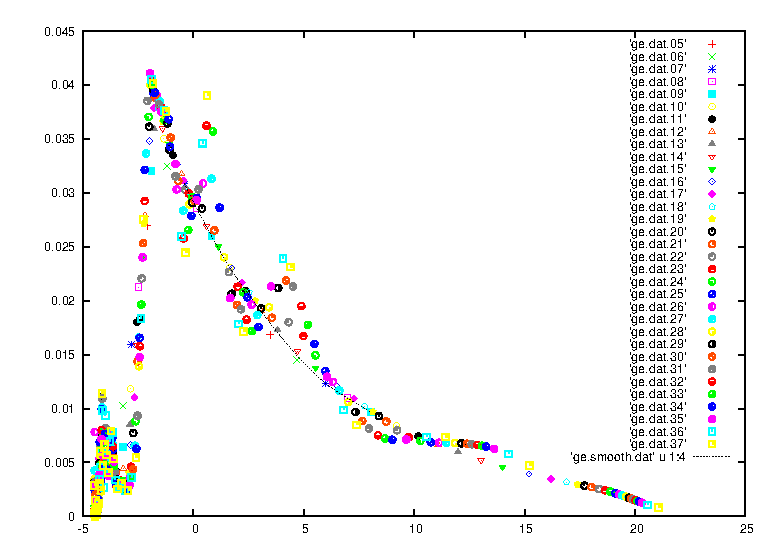
\includegraphics[scale=1.0]{pics/Xe4p_33_gammae.eps}
  \caption{$\Gamma(E)$ of the relativistic FanoADC calculation from a 4p$_{3/2}$
           initial state with both $\Gamma$ and $E$ given in atomic units.
           }
  \label{figure:Xe4p33_Gamma_profile}
\end{figure}

In case of a 4p$_{3/2}$ initial state, the decay width profile for Stieltjes
orders between 5 and 37 shows a decay
with a threshold at energies below $E_{ref}=0$, which leads to a fairly smooth
curve at the energy of interest.
At higher energies of about \unit[1.5]{a.u.} and
\unit[4.5]{a.u.} additional peaks are observed, which can be explained with
interactions of the initial state description with Rydberg states. These do not
contribute to the decay and hence a smoothing of the total curve disregarding them
is necessary.

Contrary to this, the decay width profile for the non-relativistic calculation
shown in figure \ref{figure:Xe4pnrel_Gamma_profile} illustrates several
behaviours, which indicate a very bad description of the decay widths.
The results are at this place only discussed, in order to show the necessity
of a description using relativistic quantum chemistry. The \ac{SCK} channel
is closed in this case, and therefore the channels are selected as for the
4p$_{3/2}$ initial state.

\begin{figure}[htb]
  \centering
  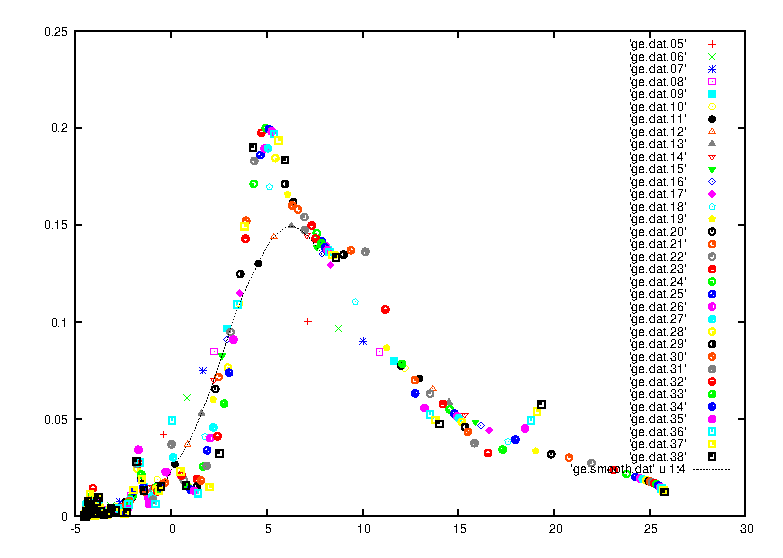
\includegraphics[scale=1.0]{pics/Xe4p_nrel_gammae.eps}
  \caption{$\Gamma(E)$ of the relativistic FanoADC calculation from a 4p$_{nrel}$
           initial state with both $\Gamma$ and $E$ given in atomic units.
           }
  \label{figure:Xe4pnrel_Gamma_profile}
\end{figure}

The most prominent issue is, that the decay width at the energy of interest
$E_{res}=0$ is not decreasing, but increasing. As illustrated in section
\ref{section:}, this behaviour can both be caused by interaction of
the initial state with Rydberg states, which do not contribute to the decay
as observed in the decay width profile of the Xe4p$_{3/2}$ initial state.
However, in this case the non-decreasing part ist not an additional feature
of a decaying curve, but rather a complete channel, which is opened at energies
above the threshold, which are included in the final state description. Such
a behaviour has in principle the physical meaning of a channel opening.
Unfortunately, the smoothing Stieltjes procedure, does not resemble a clear
cut at some threshold energy, but gives a smeared out curve where, different
orders of Stieltjes give results in a very wide range of decay widths.
Normally higher Stieltjes orders, with a higher flexibility in the polynomials give
a better approaximation than lower orders, but this can not be taken for granted.
In this particular situation, all two hole configurations included in the
final state subspace are valid final states judging from the single and
double ionization spectra of the total Hamiltonian. Therefore, the
non-relativistic results presented in table \ref{table:xe_auger_rest} can
not be trusted.

\begin{table}[h]
 \centering
 \caption{Auger decay widths of the Xe4p$_{3/2}$ and the non-relativistic
          4p. All widths are given in \unit{eV}. The non-relativistic
          results have to be handled with care, since in the calculation
          the sum over the partial decay widths is much larger, than the
          total decay width, which is not seen in this table, because
          partial widths are renormalized to the total width.}
 \begin{tabular}{lcccc}
   \toprule
                      & 4p$_{3/2,\pm 3/2}$ & 4p$_{3/2,\pm 1/2}$ & 4p$_{nrel,1}$  & 4p$_{nrel,2}$ \\
   \midrule                                                                                     
   energy [\unit{eV}] &   147.57           &    147.57          &  149.88        &   151.20    \\
   pole strength       &     0.694          &      0.694         &    0.482       &     0.209   \\
   \midrule                                                                                    
   $4d^{-2}$          &      --            &        --          &       --       &     --        \\
   $4d^{-1}5s^{-1}$   & 1.31$\cdot10^{-1}$ & 1.44$\cdot10^{-1}$ & 2.30$\cdot10^{-1}$ & 6.60$\cdot10^{-2}$\\
   $4d^{-1}5p^{-1}$   & 6.36$\cdot10^{-1}$ & 6.29$\cdot10^{-1}$ & 3.44$\cdot10^{-1}$ & 1.61$\cdot10^{-1}$\\
   $5s^{-2}$          & 6.27$\cdot10^{-4}$ & 6.29$\cdot10^{-4}$ & 3.83$\cdot10^{-4}$ & 8.65$\cdot10^{-5}$\\
   $5s^{-1}5p^{-1}$   & 1.50$\cdot10^{-2}$ & 1.49$\cdot10^{-2}$ & 3.02$\cdot10^{-2}$ & 2.07$\cdot10^{-3}$\\
   $5p^{-1}5p^{-1}$   & 3.21$\cdot10^{-2}$ & 2.90$\cdot10^{-2}$ & 5.62$\cdot10^{-3}$ & 1.42$\cdot10^{-2}$\\
   \midrule
   total              &   0.814            &   0.818            &  0.610         &   0.243     \\
   \bottomrule
 \end{tabular}
 \label{table:xe_auger_rest}
\end{table}


\begin{table}[h]
 \centering
 \caption{Auger decay widths of the Xe4p$_{3/2}$ and the non-relativistic
          partial widths are renormalized to the total width.}
 \begin{tabular}{lcccc}
   \toprule
                        & exp   & calc\footnotemark[1] & calc\footnotemark[2] & calc\footnotemark[3] \\
   \midrule                                                                         
   energy [\unit{eV}]   & 145.6 &  145.0       &  145.0       &   147.57   \\
   $\Gamma$ [\unit{eV}] &  0.54 &  1.80        &  0.3116      &  0.814\\
   \bottomrule
 \end{tabular}
 \label{table:xe_auger_comp}
\end{table}
\footnotetext[1]{\ac{MCDF} calculation excluding final ionic state configuration
                 interaction. \cite{Heinaesmaeki04}}
\footnotetext[2]{\ac{MCDF} calculation including final ionic state configuration
                 interaction. \cite{Heinaesmaeki04}}
\footnotetext[3]{This work.}


\begin{table}[h]
  \centering
  \caption{Intensity distribution for the Auger decay.}
  \begin{tabular}{lccccc}
   \toprule
                   & 4d$^{-1}$5s$^{-1}$ & 4d$^{-1}$5p$^{-1}$ & 5s$^{-2}$ & 5s$^{-1}$5p$^{-1}$ & 5p$^{-2}$ \\
   \midrule
   Ref. [\cite{Heinaesmaeki04}]\footnotemark[1] & 77.7 & 20.7  &       0.5 &       --           & 1.1     \\
   Ref. [\cite{Heinaesmaeki04}]\footnotemark[2] & 33.6 & 59.4  &       2.2 &       --           & 4.8     \\
   This work       &      16.1          &       78.1         &    0.1    &     1.8            & 3.9    \\
   \bottomrule
  \end{tabular}
  \label{table:Xe_auger_distr}
\end{table}
\footnotetext[1]{\ac{MCDF} calculation excluding final ionic state configuration
                 interaction. \cite{Heinaesmaeki04}}
\footnotetext[2]{\ac{MCDF} calculation including final ionic state configuration
                 interaction. \cite{Heinaesmaeki04}}


The Xe4p$_{1/2}$ initial state can, as already mentioned, not be described
by a single 1h configuration and therefore, all states with a pole strength
higher than 0.05 and a major contribution of the Xe4p$_{1/2}$ spinor are
investigated. Hereby, also the $4d^{-2}$ configurations are sorted into the
final state subspace in order to take care of a possible \ac{SCK} process.

Figure \ref{figure:Xe4p11_Gamma_profile} shows the decay width profile
of the lowest energy state investigated, which also inhibits the largest
pole strength. It is a inice and smooth curve at energies above $E=0$.
As can easily be seen, the \ac{SCK} decay channel opens directly
in the energy region of interest at $E_{res}=0$. Since the Stieltjes procedure
is not able to show a clear energy cut at the threshold and the initial state
energies can be expected not to be completely exact due to errors introduced
by the partitioning and additional errors from the ADC(2x) itself, an
unambiguous conclusion, whether the \ac{SCK} channel is open or not, can not be drawn.
This decission also determines the choice of which curve of the decay width
profile to choose for the evaluation of the decay width. The results shown
in table \ref{table:xe_auger_rel11} are the results for the lower curve excluding
the opening channel from the interpolation. In weighing the higher order moments
more than the lower order moments, the decay width would be about twice the numbers
presented and hence in the order of $\Gamma_{max}\unit[2]{eV}$.

\begin{figure}[h]
  \centering
  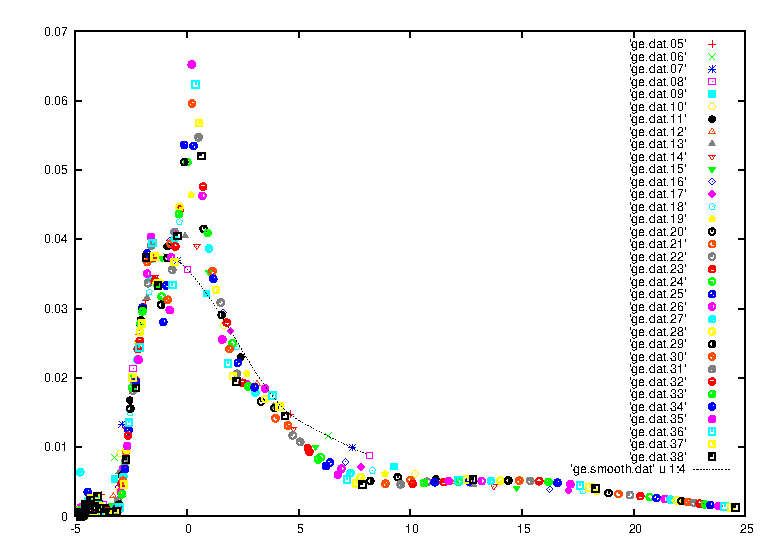
\includegraphics[scale=1.0]{pics/Xe4p_11_gammae.eps}
  \caption{$\Gamma(E)$ of the relativistic FanoADC calculation from a 4p$_{1/2}$
           initial state with both $\Gamma$ and $E$ given in atomic units.
           }
  \label{figure:Xe4p11_Gamma_profile}
\end{figure}


\begin{table}[h]
 \centering
 \caption{Auger decay widths of non-negligible satellites with a major
          contribution of the Xe 4p$_{1/2}$. All widths are given in \unit{eV}.}
 \begin{tabular}{lccccc}
   \toprule
   energy [\unit{eV}] & 156.42  & 158.16 & 160.22 & 177.77 & 186.31\\
   pole strength       &   0.332 &   0.093&   0.123&   0.058&   0.068\\
   \midrule
   $4d^{-2}$          & 6.78$\cdot10^{-1}$ & 4.45$\cdot10^{-1}$ & 1.07$\cdot10^{-1}$ & 1.68$\cdot10^{-1}$ & 1.56$\cdot10^{-1}$\\
   $4d^{-1}5s^{-1}$   & 1.34$\cdot10^{-1}$ & 6.93$\cdot10^{-2}$ & 8.61$\cdot10^{-2}$ & 1.12$\cdot10^{-1}$ & 3.39$\cdot10^{-1}$\\
   $4d^{-1}5p^{-1}$   & 2.51$\cdot10^{-1}$ & 9.08$\cdot10^{-2}$ & 1.09$\cdot10^{-1}$ & 1.45$\cdot10^{-1}$ & 3.72$\cdot10^{-1}$\\
   $5s^{-2}$          & 3.10$\cdot10^{-4}$ & 2.21$\cdot10^{-4}$ & 1.91$\cdot10^{-4}$ & 2.12$\cdot10^{-4}$ & 1.81$\cdot10^{-4}$\\
   $5s^{-1}5p^{-1}$   & 3.84$\cdot10^{-3}$ & 1.32$\cdot10^{-3}$ & 2.16$\cdot10^{-3}$ & 1.45$\cdot10^{-3}$ & 8.13$\cdot10^{-3}$\\
   $5p^{-1}5p^{-1}$   & 1.02$\cdot10^{-2}$ & 3.40$\cdot10^{-3}$ & 5.12$\cdot10^{-3}$ & 2.18$\cdot10^{-3}$ & 1.55$\cdot10^{-2}$\\
   \midrule
   total              &   1.077 &   0.610&   0.310&   0.429&   0.891\\
   \bottomrule
 \end{tabular}
 \label{table:xe_auger_rel11}
\end{table}

However, this very fast \ac{SCK} decay does not inhibit a decay width of
\unit[10--100]{eV} as estimated\cite{}. I therefore conclude, that the broad
feature of the single ionization spectrum in the 4p$_{1/2}$ region is caused
by both the breakdown of the single particle picture with additional fast decay
of all corresponding satellite configurations.


\section{Summary}
From these examples we have shown that the FanoADC Stieltjes method implemented
in Dirac is able to both reproduce results of the comparable non-relativstic
code of Koloren\v{c}  and results from \ac{MCDF} calculations
including relativistic effects in Auger processes as well as the corresponding
experimental results.
We therefore conclude that the relativistic FanoADC Stieltjes Code is able
to predict unknown decay widths for larger systems such as dimers and small
clusters.
